\documentclass[11pt,a4paper]{article} 
\usepackage[utf8]{inputenc}
\usepackage[ngerman]{babel}
\usepackage{amsmath}
\usepackage{amssymb}
\usepackage{bbm}
\usepackage{geometry}
\usepackage{graphicx}
\usepackage{verbatim}
\geometry{
  left=3cm,
  right=3cm,
  top=3cm,
  bottom=3cm,
  bindingoffset=5mm
}
\usepackage{enumerate}
\usepackage[T1]{fontenc} 
\usepackage{ucs}
\usepackage[utf8]{inputenc}
\usepackage{xcolor}

\newcommand {\Q}	{\mathbb{Q}}
\newcommand {\R}	{\mathbb{R}}
\newcommand {\C}	{\mathbb{C}}
\newcommand {\Rn}	{\mathbb{R}^n}
\newcommand {\Rzwei}	{\mathbb{R}^2}
\newcommand {\Rnxn}	{\mathbb{R}^{n \times n}}
\newcommand {\Rmxn}	{\mathbb{R}^{m \times n}}
\newcommand {\Rmxm}	{\mathbb{R}^{m \times m}}
\newcommand {\Cn}	{\mathbb{C}^n}
\newcommand {\Cnxn}	{\mathbb{C}^{n \times n}}
\newcommand {\N}	{\mathbb{N}}
\newcommand{\1}    	{\mathbbm{1}}
\newcommand{\Onot}		{\mathcal{O}}
\newcommand{\diag}	{\textrm{diag}}

\author{Ruedi Lüthi}
\title{Blatt 1}

\begin{document}

	\maketitle
	
	\section*{1.}
	
	\begin{figure}[!h]
  	\centering
 	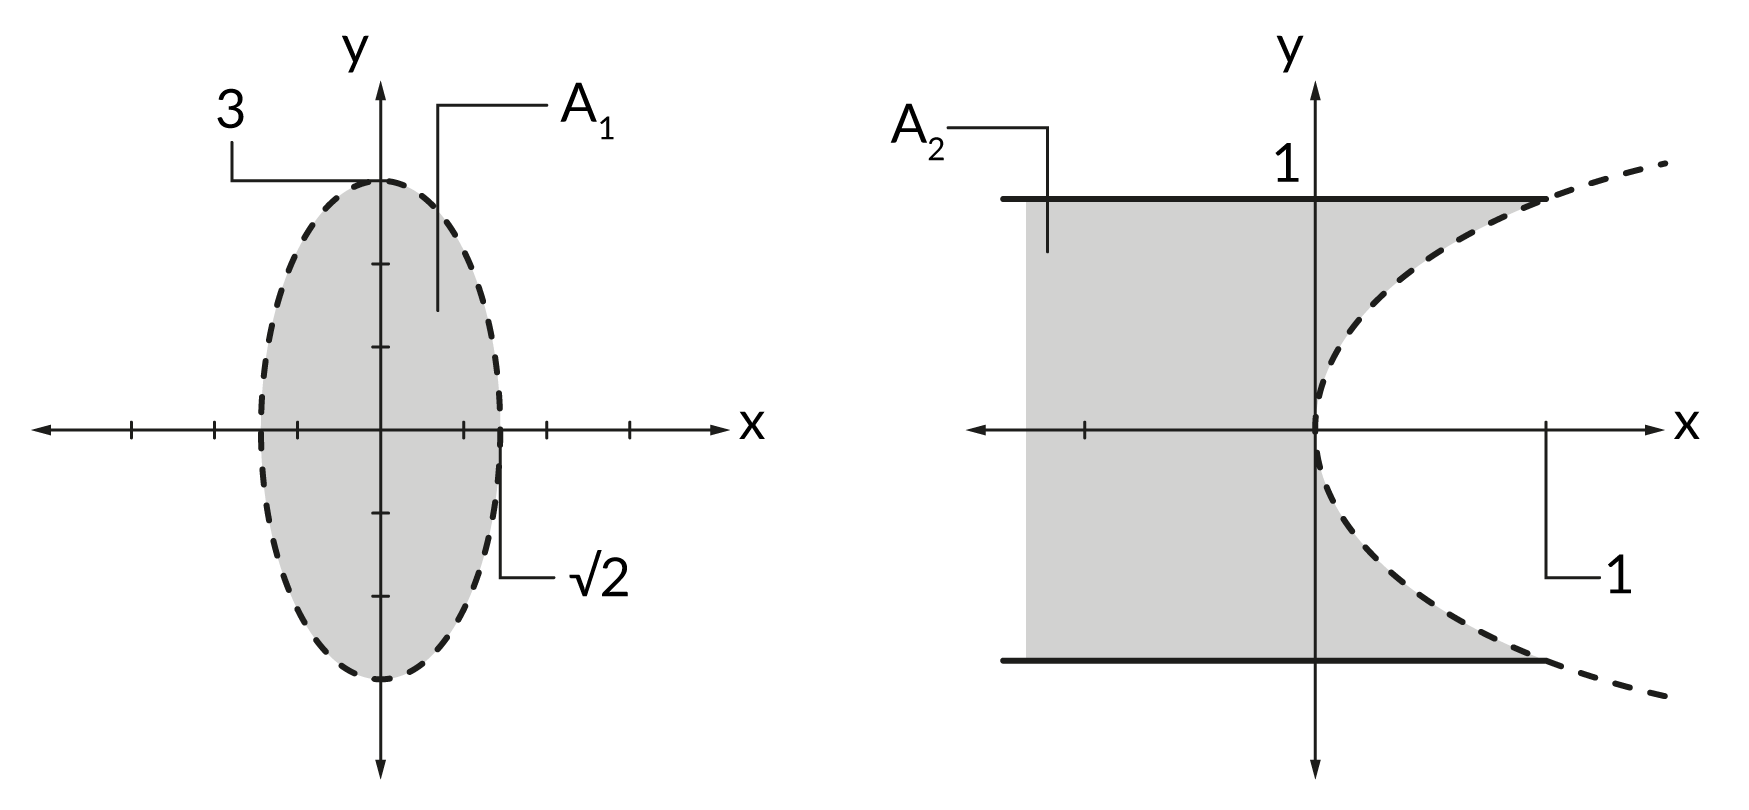
\includegraphics[width=13cm]{Blatt01_1.png}
  	\caption{Die Teilmengen \(A_1\) und \(A_2\)}
	\end{figure}

	\begin{enumerate}[i.)]
		\item
		\begin{align*}
			\mathring{A}_1 &= A \\
			\overline{A}_1 &= \left\{ \left( \begin{array}{c} x \\ y\end{array} \right) \in \Rzwei ~\right\vert \left.
			\frac{x^2}{2} + \frac{y^2}{9} \leqslant 1 \right\} \\
			\partial A_1 &= \left\{ \left( \begin{array}{c} x \\ y\end{array} \right) \in \Rzwei ~\right\vert \left.
			\frac{x^2}{2} + \frac{y^2}{9} = 1 \right\} \\
			A_1' &= \overline{A} \\
			\mathring{A}_2 &= \left\{ \left( \begin{array}{c} x \\ y\end{array} \right) \in \Rzwei ~\right\vert \left. x < y^2 ~\land~ \vert y \vert < 1 \right\} \\
			\overline{A}_2 &= \left\{ \left( \begin{array}{c} x \\ y\end{array} \right) \in \Rzwei ~\right\vert \left. x \leqslant y^2 ~\land~ \vert y \vert \leqslant 1 \right\} \\
			\partial A_2 &= 
			\left\{ \left( \begin{array}{c} x \\ y\end{array} \right) \in \Rzwei ~\right\vert \left. x = y^2 ~\land~ \vert y \vert \leqslant 1 \right\} \cup 
			\left\{ \left( \begin{array}{c} x \\ y\end{array} \right) \in \Rzwei ~\right\vert \left. \vert y \vert = 1 ~\land~ x \leqslant 1 \right\} \\
			A_2' &= \overline{A}
		\end{align*}
		\item \(A_1\) ist offen, \(A_2\) nicht
		\item \(A_1, A_2\) sind nicht abgeschlossen
		\item \(A_1\) ist beschränkt, \(A_2\) nicht
	\end{enumerate}
	
	\section*{2.}	
	
	Sei \(\mathcal{O}_j \subset \Rn\) eine beliebige abgeschlossene Menge. Nun wissen wir nach Satz 1.1.7, wenn \(\mathcal{O}_j\) abgeschlossen ist, dass das Komplement \((\mathcal{O}_j)^c\) offen ist. Also gilt für die Vereinigung der Komplemente zweier offene Mengen \(\mathcal{O}_1, \mathcal{O}_2 \) nach den De Morganschen Gesetzen:
	\begin{align*}
		A = (\mathcal{O}_1)^c \cup (\mathcal{O}_2)^c \quad\Leftrightarrow\quad \left( \mathcal{O}_1 \cap \mathcal{O}_2 \right)^c = A
	\end{align*}
	Weiter wissen wir wegen Satz 1.1.8, dass die Vereinigung zweier beliebigen offener Mengen wiederum offen ist, also muss \(A\) offen sein.
	Wiederum nach Satz 1.1.7 ist das Komplement \(A^c\) aber abgeschlossen:
	\begin{align*}
		A^c = \left( \left( \mathcal{O}_1 \cap \mathcal{O}_2 \right)^c \right)^c = \mathcal{O}_1 \cap \mathcal{O}_2
	\end{align*}
	und somit also auch der Durchschnitt der abgeschlossenen Mengen \(\mathcal{O}_1, \mathcal{O}_2 \). \\
	\\
	\noindent
	Die Behauptung für beliebig viele Mengen folgt wiederum über Induktion:
	\begin{align*}
		A = \mathcal{O}_1 \cap \underbrace{\left( \mathcal{O}_2 \cap \mathcal{O}_3 \cap ... \cap \mathcal{O}_n \right)}_{\mathcal{O}'_2} 
	\end{align*}
	
	\section*{3.}
	\subsection*{a)}
	Betrachten wir die Funktion \(f\) für \(x \neq 0\) und \(y \neq 0\) und transformieren in Polarkoordinaten \(x = r \cos \phi, y = r \sin \phi \):
	\begin{align*}
		f(x,y) = \frac{xy}{x^2 + y^2} = \frac{r \cos \phi \cdot r \sin \phi}{r^2 \cos^2 \phi + r^2 \sin^2 \phi} = \frac{\cos \phi \sin \phi}{ \cos^2 \phi + \sin^2 \phi} = \cos \phi \sin \phi = f(r,\phi)
	\end{align*}
	Weiter betrachten wir:
	\begin{align*}
		\lim_{r \rightarrow 0} f(r,\phi) =\cos \phi \sin \phi 
	\end{align*}
	Da \(\lim_{r \rightarrow 0} f \left( r,\frac{\pi}{4} \right) = \frac{1}{2} \neq 0 = \lim_{r \rightarrow 0} f( r, \pi ) \) kann die Funktion \underline{nicht stetig} sein.
	
	\subsection*{b)}
	Mit \textbf{\(\varepsilon\)-\(\delta\)-Kriterium} (nach \underline{Musterlösung}): \\
	\textit{Bemerkung}: Seien \((M_1,d_1)\) und \((M_2,d_2)\) zwei metrische Räume und \(D \subset M_1\). So ist eine Funktion \(f: D \rightarrow M_2\) genau dann stetig in \(a \in D\), wenn zu jedem \(\varepsilon > 0\) ein \(\delta_\varepsilon > 0\) existiert, so dass für \(x \in D\) gilt \(d_1(x,a) < \delta_\varepsilon \rightarrow d_2(f(x), f(a)) < \varepsilon\).
	\begin{align*}
		\forall~ \varepsilon > 0 \quad \exists~ \delta_\varepsilon > 0 \quad:\quad d_1(x,a) < \delta_\varepsilon \rightarrow d_2(f(x), f(a)) < \varepsilon \quad \forall~ x \in D
	\end{align*}
	Sei \(\varepsilon > 0\) beliebig und \(\delta_\varepsilon = \frac{\varepsilon}{2}\) sowie \(x = \left( \begin{array}{c} x \\ y \end{array} \right) \in U_{\delta_\varepsilon}( 0 )\). Dann gilt für \(g(x)\) stetig:
	\begin{align*}
		\left\Vert \left( \begin{array}{c} x \\ y \end{array}\right)\right\Vert < \delta_\varepsilon
		\quad&\Rightarrow\quad \left\{ \begin{array}{c}
			\vert x \vert < \delta_\varepsilon \\
			\vert y \vert < \delta_\varepsilon
		\end{array} \right. \\
		\left\vert f(x,y) - f(0,0) \right\vert &= 
		\left\vert \frac{x^5 - y^5}{x^4 + y^4} - 0 \right\vert \stackrel{\Delta\textrm{-Ungleichung}}{\leqslant} \frac{\vert x \vert ^5}{x^4 + y^4} + \frac{\vert y \vert ^5}{x^4 + y^4} \\
		&\stackrel{\substack{x \neq 0 \\ y \neq 0}}{=} \vert x \vert \frac{1}{1 + \frac{y^4}{\vert x \vert^4}} + \vert y \vert \frac{1}{\frac{x^4}{\vert y \vert^4} + 1} \leqslant \underbrace{\vert x \vert}_{< \delta_\varepsilon} +  \underbrace{\vert y \vert}_{< \delta_\varepsilon} < 2 \delta_\varepsilon = \epsilon
	\end{align*}
	
	\noindent	
	Mit \textbf{Folgenkriterium} (entspricht \underline{nicht} der Musterlösung): \\
	\color{red} Dies beweist die Stetigkeit \underline{nicht}! Sondern lediglich die Konvergenz von \(f(x_n,\phi)\). \\
	\color{black}
	Dasselbe
	\begin{align*}
		f(x,y) = \frac{x^5 - y^5}{x^4 + y^4} = \frac{r^5 ( \cos^5 \phi - \sin^5 \phi )}{r^4 ( \cos^4 \phi + \sin^4 \phi) } = r \frac{\cos^5 \phi - \sin^5 \phi}{\cos^4 \phi + \sin^4 \phi} = f(r,\phi)
	\end{align*}
	wiederum
	\begin{align*}
		& \lim_{r \rightarrow 0} f(r,\phi) \quad\textrm{oder}\quad
		\lim_{n \rightarrow \infty} f\left( x_n,\phi \right) \quad\textrm{mit}\quad
		(x_n) = \frac{\cos^4 \phi + \sin^4 \phi}{n} \\
		& \lim_{n \rightarrow \infty} \frac{\cos^4 \phi + \sin^4 \phi}{n} < \lim_{n \rightarrow \infty} \frac{2}{n} = 0 \quad \textrm{(Nullfolge)} \\
		& \lim_{n \rightarrow \infty} f\left( x_n,\phi \right)  = 
		\lim_{n \rightarrow \infty} \frac{\cos^4 \phi + \sin^4 \phi}{n} \frac{\cos^5 \phi - \sin^5 \phi}{\cos^4 \phi + \sin^4 \phi} = 
		\lim_{n \rightarrow \infty} \frac{1}{n} (\cos^5 \phi - \sin^5 \phi) < \lim_{n \rightarrow \infty} \frac{2}{n} = 0
	\end{align*}
	Da \( \lim_{n \rightarrow \infty} f\left( x_n,\phi \right) = 0\) und \(f( x_0) = 0\) ist die Funktion \underline{stetig}.
	
	\section*{4.}
	\subsection*{a)}
	Für das Zeichnen der Höhenlinie mit Wert \(c\) stellen wir um:
	\begin{align*}
		f(x,y) = 4x^2 - 9y^2 = c \quad &\Leftrightarrow \quad y^2 = \frac{4x^2 - c}{9} \\
		&\Rightarrow \quad y_{1,2} = \pm \frac{1}{3} \sqrt{4x^2 - c} = h(x,c)
	\end{align*}
	und zeichnen mittels der Funktion \(h(x,c)\) diese im entsprechenden Definitionsbereich \(\left\{ x \in \left[ -1, 1 \right] : 4x^2 - c > 0 \right\} \):
	
	\begin{figure}[!h]
  	\centering
 	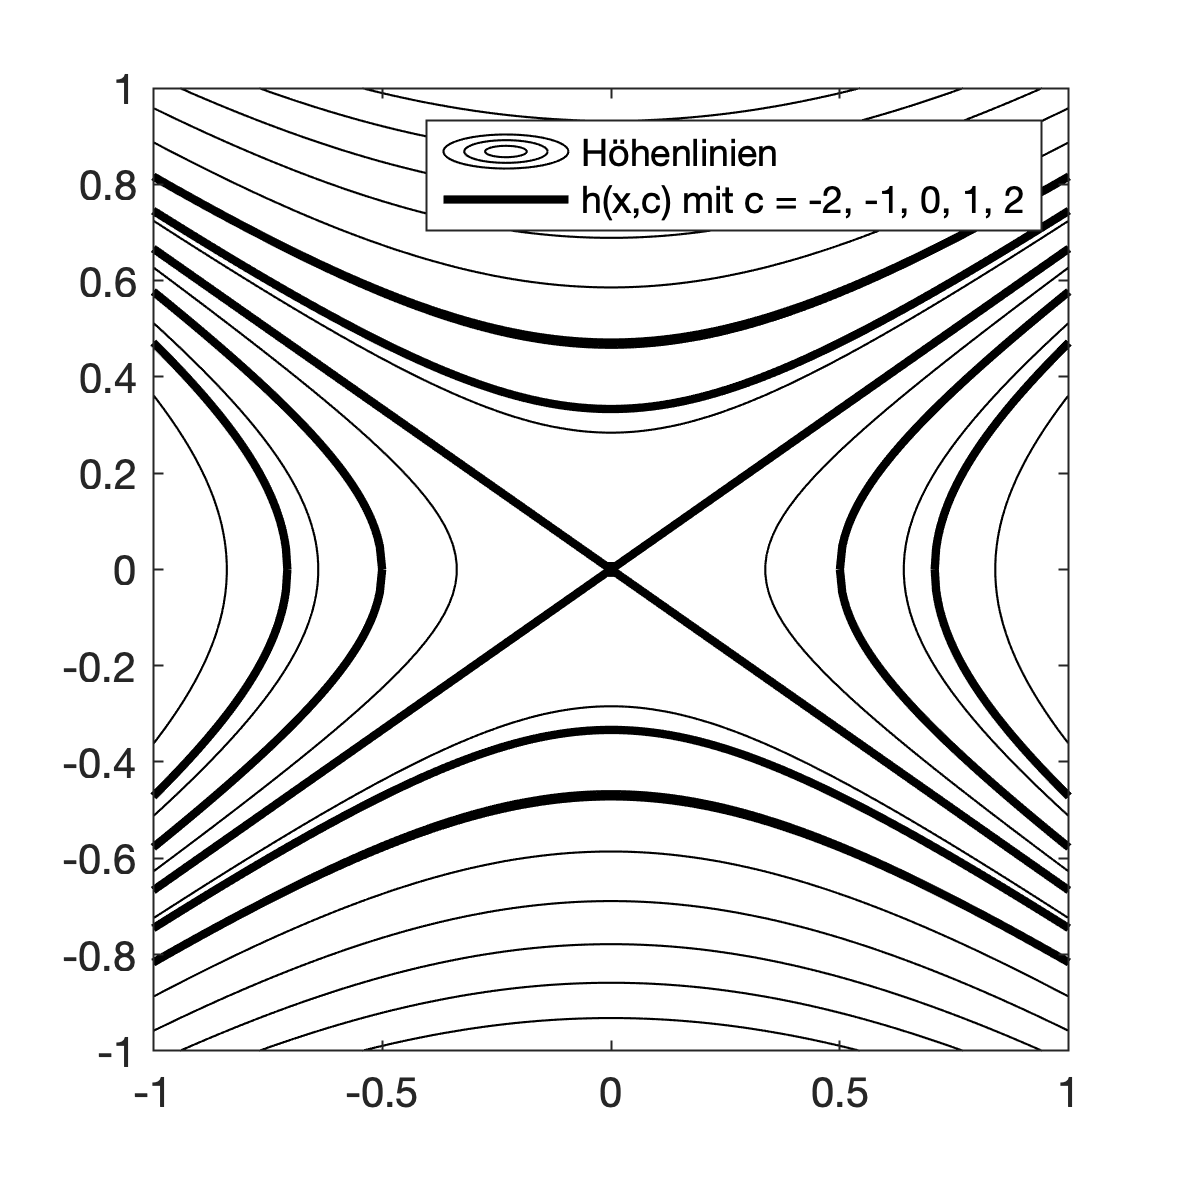
\includegraphics[width=10cm]{Blatt01_4a.png}
  	\caption{Die Höhenlinien der Funktion \(f(x,y)\) }
	\end{figure}
	
	\subsection*{b)}
	
	Partiell ableiten:
	\begin{align*}
		\nabla f(x,y) = \left( \begin{array}{ccc}
			frac{\partial}{\partial x} 4x^2 - 9y^2 & = & 8x \\
			\frac{\partial}{\partial y}  4x^2 - 9y^2 & = & -18y
		\end{array} \right)
	\end{align*}
	
	\begin{figure}[!h]
  	\centering
 	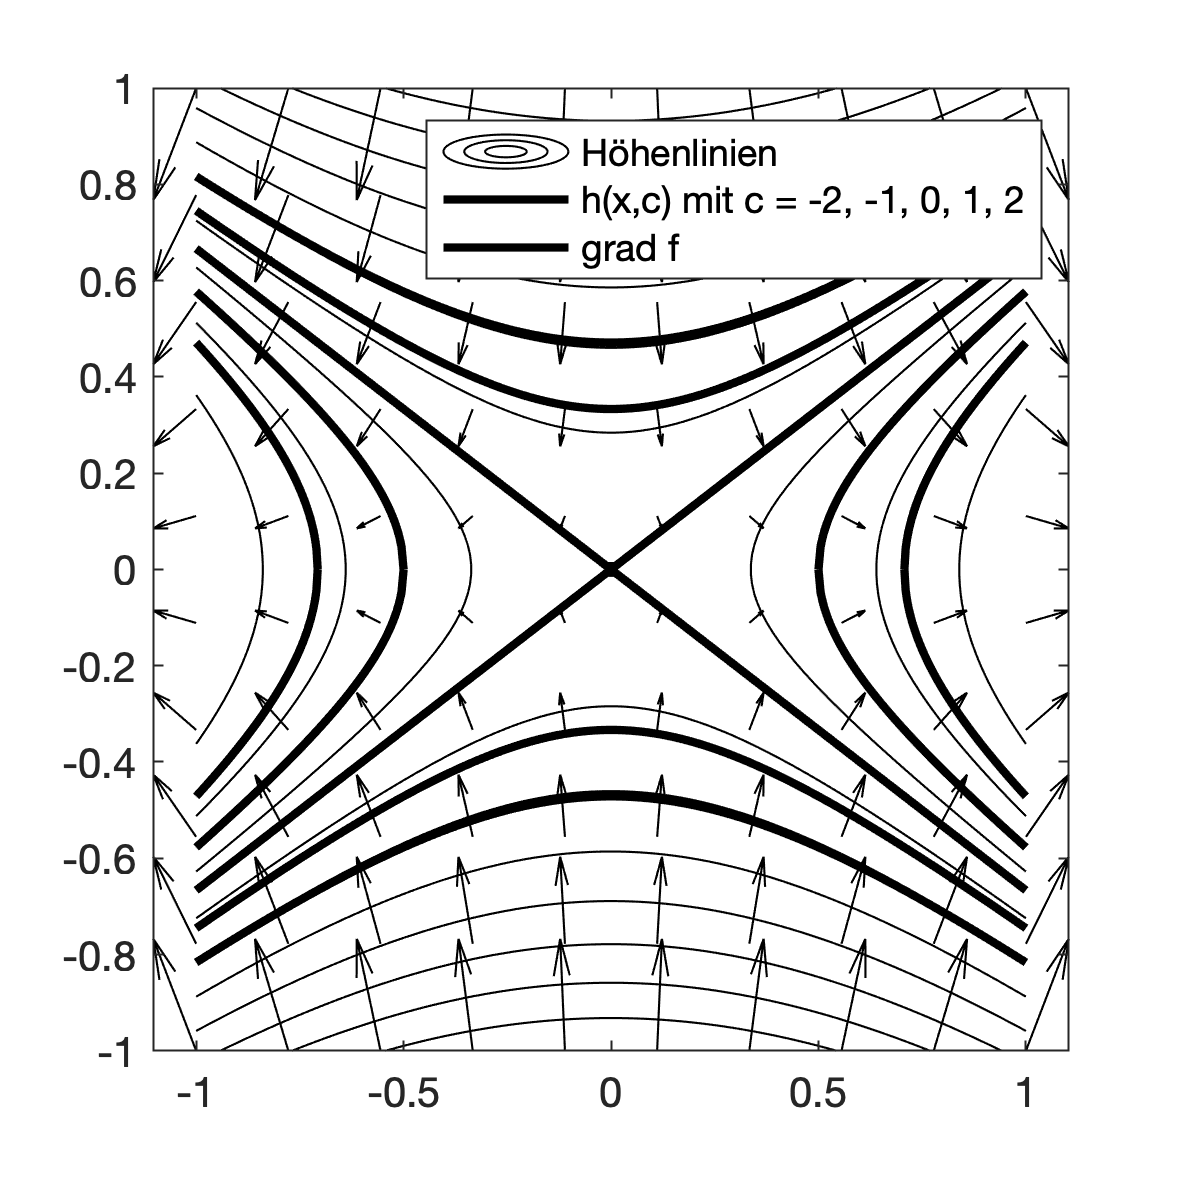
\includegraphics[width=10cm]{Blatt01_4b.png}
  	\caption{Vektorfeld \(\nabla f(x,y)\) }
	\end{figure}
	
	
\end{document}